\status{started}
\chapter{Liquid Hydrogen target}
\label{ch:MEG:CEX}
\begin{refsection}
{\itshape In this chapter the Charge EXchange reaction, a calibration for the liquid XEnon Calorimeter, will be discussed and an in-depth description of the associated Liquid Hydrogen Target is given. 
Data taking, analysis, performances, and the different modifications will be also discussed.
This target was designed in 2020 to overcome some limitations of the previous and in the last two years went through some heavy re-development.
This calibration is cardinal for the correct functioning of the key subdetector of the MEG II experiment. It  was one of the main tasks in my involvement in this experiment and it absorbed a sizable portion of my time and effort.}

\status{started} 
\section{Charge EXchange reaction}
    As already discussed, the $\upmu \rightarrow e\upgamma$ process searched by MEG leads to a monochromatic photon at \SI{53.2}{MeV}.
    We saw in Sec.~\ref{sec:cw:calib} the XEC calibration which is performed three times a week. 
    Unfortunately, while the frequent calibrations are great for the time dependencies, the photon produced by the \ce{Li} is at lower energy than the signal.
    To calibrate the calorimeter near the signal region, the Charge EXchange reaction is exploited.
    The Charge EXchange (CEX) process $\pi^-p\rightarrow \pi^0n$; $\pi^0\rightarrow\gamma\gamma$ produces $\gamma$ with a flat distribution in the interval $[54.9,82.9]$ MeV.
    Extremal values are reached for photons emitted back to back. Thus, a signal-like photon can be tagged by detecting a high-energy photon in the opposite direction.
    The tagging is performed with a BGO detector which can be positioned (steps of 30 cm in \^{z} and 16 deg in $\hat{\varphi}$) opposite to specific \textit{patches} of the XEC.
    The requirement $\Delta E/E< 1\%$ translates to $\Delta \theta_{\gamma\gamma}<5^\circ$.
    A sketch of the CEX measurements, a picture of the BGO detector, and its moving structure is shown in Fig.~\ref{fig:CEX}.

    \newcommand\h{5cm}
    \begin{figure}[ht]   
    \centering
        \subfloat[CEX sketch]{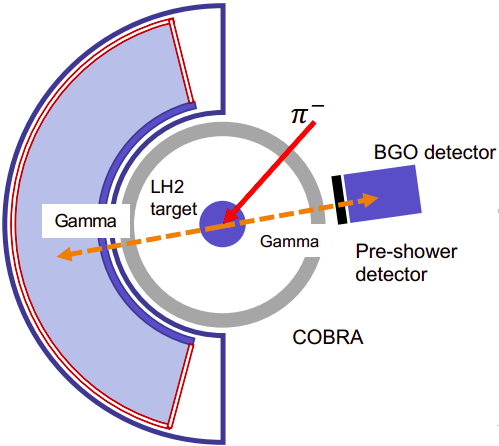
\includegraphics[height=\h, keepaspectratio]{Figures/LH2/CEX_sketch.png}\label{fig:CEX:sketch}}
        \subfloat[BGO crystals]{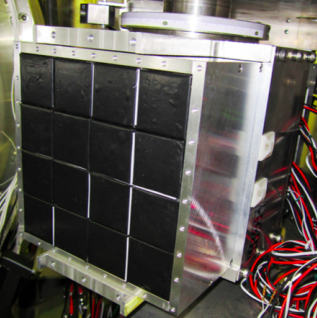
\includegraphics[height=\h]{Figures/LH2/BGO.png}\label{fig:CEX:bgo}}
        \subfloat[BGO mover]{
        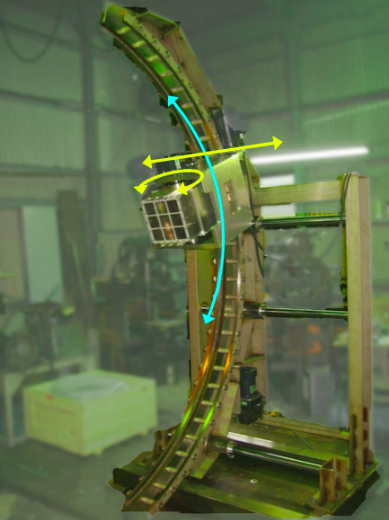
\includegraphics[height=\h, keepaspectratio]{Figures/LH2/BGO_mover.png}\label{fig:CEX:mover}}
        \caption{Diagram of the CEX measurement, with the back-to-back photons configuration to define the XEC patch via the BGO positioning (\ref{fig:CEX:sketch}) Picture of the BGO detector (\ref{fig:CEX:bgo}) Picture of the BGO mover (\ref{fig:CEX:mover}).}
        \label{fig:CEX}
    \end{figure}

\status{started}
\section{BGO}
    The BGO crystal already mentioned, and shown in Fig.~\ref{fig:CEX:bgo}, is an auxiliary detector that plays a key role in two subjects of this thesis.
    For this reason, we will here describe it in some detail.
    BGO refers to \ce{Bi4Ge3O12}, a compound with a cubic crystal structure and often used as a scintillator.
    This detector is, in particular, a matrix 4x4 of \SI{4x4}{cm} crystals and mounted on a structure (see Fig.~\ref{fig:CEX:mover}) that allows it to translate and rotate around COBRA.

\status{started}
\section{LH2 target working principle}
    The details of the circuit and the operation changed on a yearly basis but it's worth do discuss the overall working principle before seeing the evolution of this system.
    Liquid Hydrogen was chosen to provide the protons needed for the CEX reaction.  
    The incoming 70.6 MeV/c $\pi^-$ are stopped in a cylindrical cell (60 mm diameter, 70 mm length) of 0.5 mm stainless steel containing liquid Hydrogen. 
    This corresponds to $\sim 90\%$ stopping efficiency.
    The hydrogen has to be kept liquid ($T<20.39$ K at 1 atm) and in the center of the COBRA magnet, requiring a cryogenic infrastructure to be inserted for 2 m.
    The target consists of four sub-systems:
    \begin{itemize}
        \item A ``closed volume'' hydrogen circuit, in which a $1.5$ bar over-pressurized $100\ \ell$ buffer is connected to the target cell 
        \item  A copper rod (2 m in length and 2 cm in diameter): supported and cooled at one end with liquid helium flowing in a copper coil; holding the target cell at the other.
        \item Vacuum Insulation for the whole system
        \item A slow-control based on an SCS2000 \cite{midas} controlling: temperatures, pressures, He flux, and the alarm system
    \end{itemize}
    The buffer volume for the gaseous hydrogen, as well as all the infrastructure and services, are kept outside the magnet. The circuit for the 2021 version is shown in Fig. \ref{fig:LH2:2021:circuit} and, to increase the readability, the different sub-circuits are color-coded:
    \begin{itemize}
        \item Blue - Hydrogen is filled into the buffer from a cylinder, which gets then removed.
        The buffer itself is connected to the cell, the exhausting line, a vacuum pump, piezoresistive pressure transmitters and a Nitrogen bottle
        \item Red - The liquid He flux is obtained by pressurizing a Dewar with an He bottle. 
        The He passes around the Cu rod and through a heater before entering the He recovery line
        \item Green - Insulation vacuum system
        \item Yellow - A nitrogen bottle is used for purging the hydrogen when emptying the buffer and kept connected for safety
    \end{itemize}

    \begin{sidewaysfigure}
        \centering
        \includegraphics[width=\textwidth]{Figures/LH2/2021/2021_LH2_circuit.png}
        \caption{Circuit of the LH2 target. To increase the readability of the scheme of the circuit, the different sub-circuits are color-coded:\\ Blue - Hydrogen; Red - Liquid Helium; Green - Insulation vacuum; Yellow - A nitrogen}
    \label{fig:LH2:2021:circuit}
    \end{sidewaysfigure}

    \status{started}
    \subsection{Operation and control}
        The operation of the target itself is partially manual and partially controlled through a LabVIEW program which, for example, controls the read-out of the various sensors and the flux of the incoming He. 
        A module SCS2000 allows to read the various sensors. 
        There are two key indicators used to monitor the liquefaction process and stability of the system:
    
        \begin{itemize}
            \item Temperature sensors: resistors(later replaced by Lakeshore silicon diodes sensors) have been put in thermal contact with the Cu rod at both ends (two per side for redundancy). 
            The readings of these elements allow us to monitor the cooling at the Cu coil and the cell.
            \item Hydrogen pressure: at room temperature, the hydrogen is set to 1.5 bar over-pressure. When the liquefaction starts the overall pressure is reduced and can be linked to the amount of liquid Hydrogen in the cell. 
        \end{itemize}

\status{started}
\section{2021}
    I started my Ph.D in November 2020 but I joined the activities after the first year, in October 2021. 
    For this reason, I did not participate in the development of the first iteration of the target and I joined directly the first tests before the data taking period.
    The status of the LH2 Target and the preliminary results of the 2021 CEX were presented at the 15th Pisa Meeting on Advanced Detectors \cite{Elba:mio}.

    \status{started}
    \subsection{Data taking}
        The data taking lasted roughly two weeks, during which CR runs and XEC calibrations were run while the target was cooling and liquefying. 
        As soon as the level was sufficient the pion beam would be used for CEX data taking for a specific patch of the XEC.  
        When the dewar needed to be exchanged, the data taking would be stopped and CR/calibrations would restart, waiting for the target to be sufficiently full to restart.
        \noindent
        In figure \ref{fig:CEX:2021:datataking} is shown the history of the Hydrogen and Helium pressure at the dewar. 
        Interesting features are:
        \begin{outline}
            \1 The decreasing parts of the blue plot are the liquefaction period: the Hydrogen pressure drops because of the phase change
            \1 During liquefaction, some spikes can be seen: these are instances in which the system became unstable and liquefaction stopped
            \1 The speed of cooling and liquefaction is always the same because the result of hardware choices; 
        \end{outline}
        Overall, CEX data could be collected when the target was considered `full enough': below AAA bar, meaning \SI{0}{\%}. 
        In the two weeks, this translates to efficiency of $\varepsilon_{2021}\approx0$.
        The efficiency for 2021 was lower than expected and the necessary statistic was not reached for every patch.
        
        \begin{figure}
            \centering
            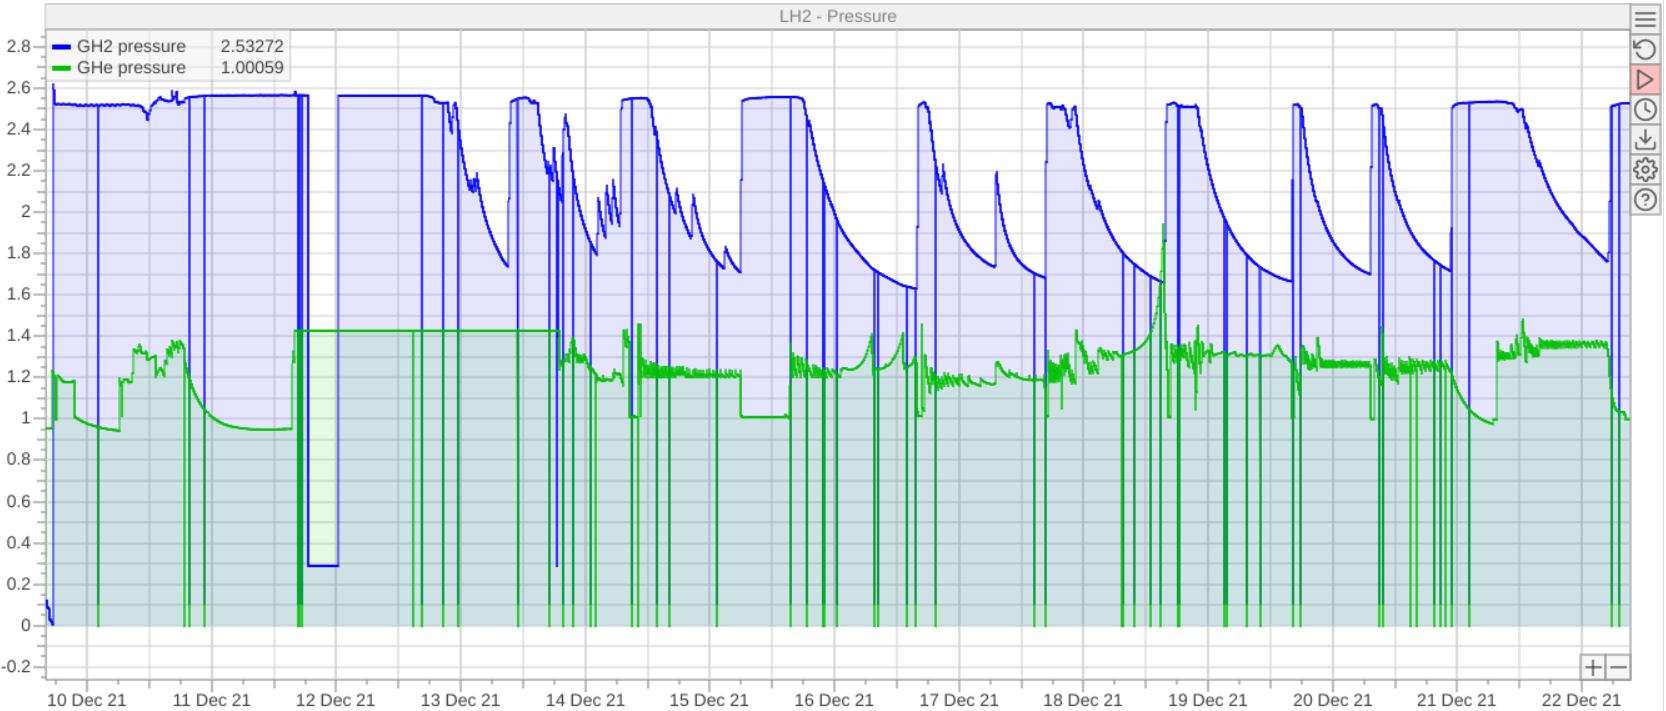
\includegraphics[width = \textwidth]{Figures/LH2/2021CEX_LH2.png}
            \caption{Measured hydrogen pressure in the target and helium pressure in the dewar used for cooling during 2021 CEX data taking. 
            Beam was ON when the target was considered `full enough': below AAA bar, meaning \SI{0}{\%}. 
            This translates to a time efficiency of $\varepsilon_{2021}\approx0$. 
            Unfortunately, the low efficiency prevented the collection of the necessary statistics for every patch of the XEC.}
            \label{fig:CEX:2021:datataking}
        \end{figure}
    
    \subsection{Data anlaysis}

\section{2022}
    \subsection{Upgrades}
        \paragraph{He circuit}
        \paragraph{Cup}
        \paragraph{Shielding}
        
    \subsection{Data taking}
        \begin{figure}
            \centering
            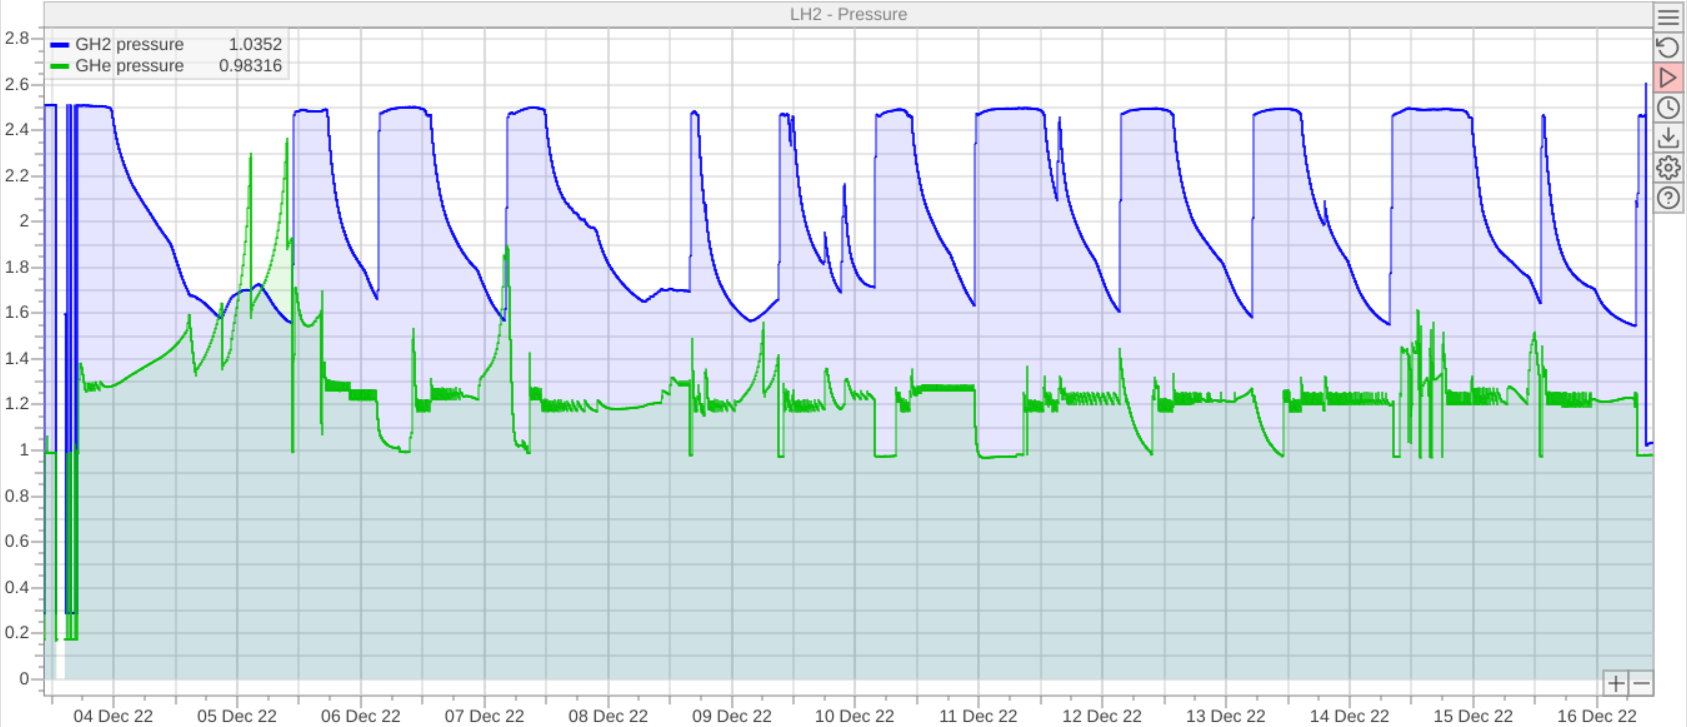
\includegraphics[width = \textwidth]{Figures/LH2/2022CEX_LH2.png}
            \caption{Measured hydrogen pressure in the target and helium pressure in the dewar used for cooling during 2022 CEX data taking. 
            Beam was ON when the target was considered `full enough': below AAA bar, meaning \SI{0}{\%}.  
            This translates to a time efficiency of $\varepsilon_{2022}\approx0$ (against $\varepsilon_{2021}\approx0$). 
            The improvement in efficiency allowed us to collect the necessary statistics for every patch of the XEC.}
            \label{fig:CEX2022}
        \end{figure}

    \subsection{Data analysis}

\section{2023}
    Although the 2022 CEX campaign was much more successful than the previous one, the limitations of this design and the second iteration dictated a hectic schedule during data taking. 
    The (somewhat risky) modification of the liquid hydrogen cup turned out to be a good improvement but there was still room for refinement. 
    For this reason, we went back to the drawing board.

    \subsection{Upgrades}
        \paragraph{He circuit}
        \paragraph{Cup}
        \paragraph{Shielding}
    \subsection{Data taking}
    \subsection{Data anlaysis}

\section{Conclusions}

\status{started}
\printbibliography[
    heading = bibliographychapter,
    title=Bibliography on \ce{LH2}
]

\end{refsection}
